\documentclass{article}
\usepackage{amsmath, amssymb, mathtools, bm}
\usepackage{graphicx, graphics}
\DeclareMathOperator*{\argmin}{arg\,min}

\title{PyKE: Open source Python data analysis for NASA's Kepler, K2, and TESS missions}
\author{PyKE Contributors}
\date{\today}

\begin{document}
\maketitle

\begin{abstract}

\end{abstract}

\section{Introduction}

\section{Lightcurve Basics}
    \subsection{The \texttt{LightCurve} class}
        A \texttt{LightCurve} object can be instantiated by passing a \texttt{time}
        array, a \texttt{flux} array, and optionally a \texttt{flux\_err} array which
        accounts for uncertainties in the \texttt{flux} measurements.
        \begin{verbatim}
        from pyke.lightcurve import LightCurve
        lc = LightCurve(time, flux)
        \end{verbatim}

        Once instantiated, a \texttt{LightCurve} object provides methods such
        as:
        \begin{description}
            \item[\texttt{stitch}]: appends the attributes \texttt{flux},
                \texttt{time}, and \texttt{flux\_err} of other given
                \texttt{LighCurve} objects.
            \item[\texttt{flatten}]: applies a Savitzky-Golay filter to capture
                low frequency flux variations which can be then removed in order
                to aid transit detection algorithms.
            \item[\texttt{fold}]: folds a lightcurve at a given period and
                phase.
            \item[\texttt{bin}]: bins a lightcurve using a block mean or median.
            \item[\texttt{cdpp}]: computes the Combined Differential Photometric
                Precision (CDPP) metric, which is a proxy for the amount of
                scatter in the lightcurve signal.
            \item[\texttt{plot}]: plots a lightcurve in a user-friendly fashion.
        \end{description}

       The \texttt{KeplerLightCurve} class extends \texttt{LightCurve} by
       adding attributes to store metadata information such as channel number,
       quality flags, campaign or quarter number, kepler id, etc.

       Additionally, \texttt{KeplerLightCurve} can be corrected for motion-dependent
       correlated noise using the \texttt{correct} method which will be discussed in
       Section~\ref{subsection:motion}.

   \subsection{The \texttt{KeplerLightCurveFile} class}
        The \texttt{KeplerLightCurveFile} class defines a structure to deal
        with lightcurve files from both NASA's Kepler and K2 missions.

        To instantiate a \texttt{KeplerLightCurveFile} object, it is necessary
        to pass a \texttt{path} which represents the address (url or local path)
        of a lightcurve file in the fits (or compressed) format, and a
        \texttt{quality\_bitmask} string which specifies quality
        flags of cadences that should be ignored.

        One crucial method of the \texttt{KeplerLightCurveFile} class is
        \texttt{get\_lightcurve} which returns a \texttt{KeplerLightCurve} object
        with the metadata provided by the corresponding \texttt{KeplerLightCurveFile}.

        Therefore, one can, for example, perform the following series of operations
        in order to fold a lightcurve from the MAST archive
        \begin{verbatim}
        lc_file = KeplerLightCurveFile(path=PATH_TO_FILE)
        klc = lc_file.get_lightcurve("PDCSAP_FLUX").fold(period=10.8234)
        klc.plot()
        \end{verbatim}
        [use a real example here]

\section{Target Pixel File Basics}

\section{Tools}

\subsection{Cotrending basis vectors}

Cotrending basis vectors (CBVs) correction consists in removing global correlated
systematics that occurs in a given channel [add reference]. The procedure of
designing the CBVs is discussed in [add reference].

Briefly, given a set of $n$ CBVs, one is interested in finding a set of $n$
coefficients $\bm{\theta}=(\theta_1, \theta_2, ..., \theta_n)$ which minimizes
some cost function between the SAP flux and the set of CBVs.

The following cost function is often used
\begin{align}
    \bm{\theta}^{*} = \argmin_{\bm{\theta} \in \Theta} \sum_{t}|f_{SAP}(t)
    - \sum_{j=1}^{n}\theta_j v_{j}(t)|^p, p>0, p \in \mathbb{R},
\end{align}
in which $f_{SAP}$ is the SAP flux and $v_j$ is the $j$-th CBV.

Then, the cbv-corrected flux can be computed as
\begin{equation}
    f_{CBV} = f_{SAP} - \sum_{j=1}^{n}\theta^{*}_j v_{j}(t).
\end{equation}

A runnable example of SAP flux correction for target \texttt{KOI 8462852}
can be written as follows
\begin{verbatim}
from pyke.lightcurve import KeplerCBVCorrector
cbv = KeplerCBVCorrector("https://archive.stsci.edu/missions/kepler/lightcurves/"
                         "0084/008462852/kplr008462852-2011073133259_llc.fits")
cbv_lc = cbv.correct(cbvs=[1,2])
\end{verbatim}

As a result, Fig~\ref{fig:cbv-correction} illustrates the correction.
\begin{figure}[!htb]
    \centering
    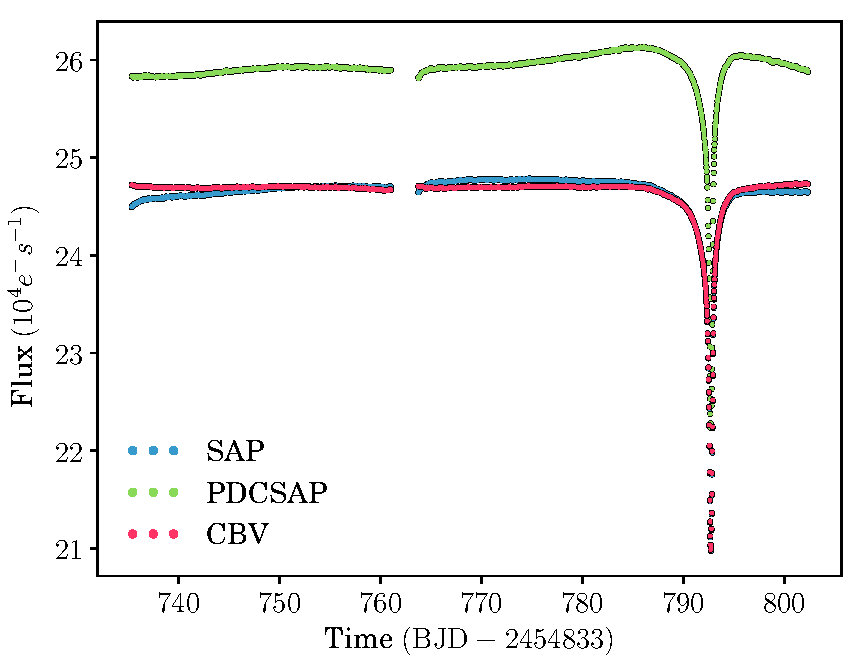
\includegraphics[scale=.5]{figs/cbv.pdf}
    \caption{CBV correction applied on \texttt{KOI 8462852}}
    \label{fig:cbv-correction}
\end{figure}

In this setting, the user is left to choose the cost function and the number
of CBVs. It is often the case where $p=1$ yields robust (non-overfitted) results.
In fact, $p=1$ defines the $\ell_1$-norm which is robust against outliers [add reference].

The number of CBVs will directly contribute to overfitting effects. One
way to identify a reasonable number of CBVs is to perform a grid search
as suggested in Fig~(\ref{fig:cbv-grid-search}).

\begin{figure}[!htb]
    \centering
    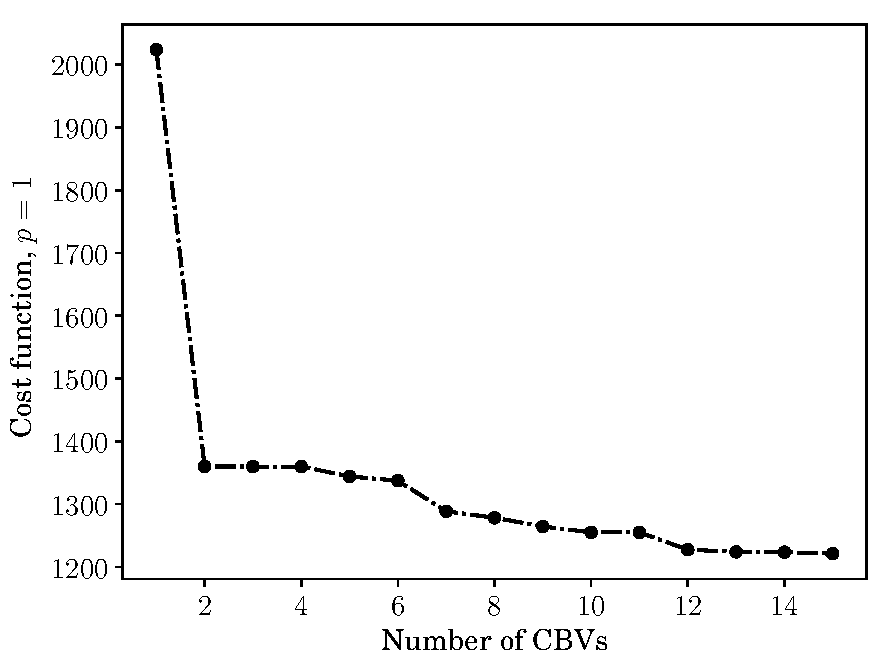
\includegraphics[scale=.5]{figs/cbv-grid-search.pdf}
    \caption{Grid search on the number of CBVs}
    \label{fig:cbv-grid-search}
\end{figure}

In the same fashion, we can apply cotrending basis vector correction to
\mathcal{K}\mathit{2} lightcurves.

For example, Fig.~\ref{fig:cbv-correction-k2} shows the result after estimating
the first nine coefficients for CBV correciton on target \texttt{EPIC 201543306}.
The selection of the number of CBVs is also done empirically by inspecting the
grid search curve.
\begin{figure}[!htb]
    \centering
    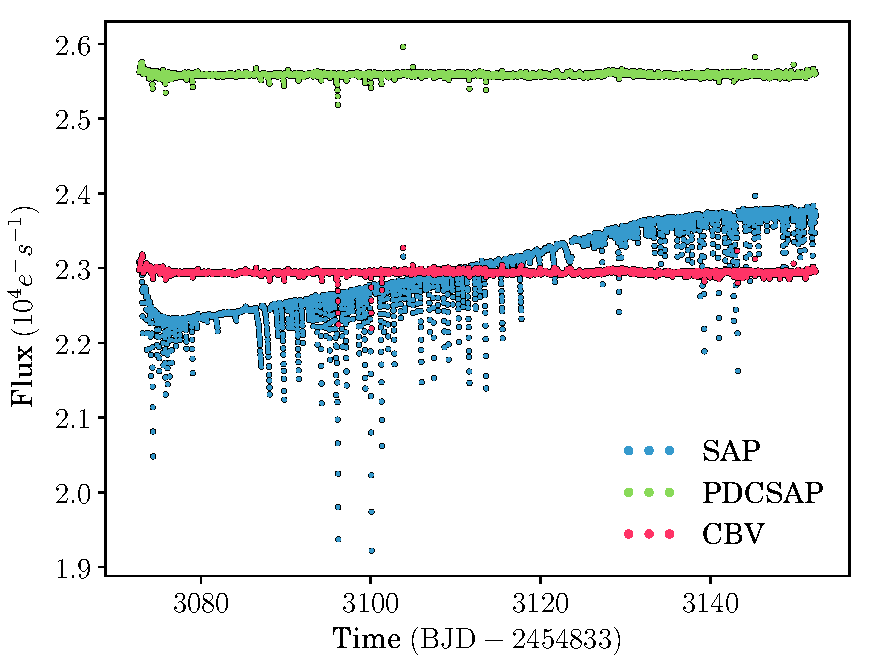
\includegraphics[scale=.5]{figs/cbv-k2.pdf}
    \caption{CBV correction applied on \texttt{EPIC 201543306}.}
    \label{fig:cbv-correction-k2}
\end{figure}

\subsection{Point spread function photometry}

PyKE contains routines to perform PSF photometry in TPFs
which are implemented in the \texttt{psf} module.

Briefly, the PSF photometry problem that PyKE solves can be formulated as
follows. Given an image $\bm{y}$, with $n$ pixels and $m$ stars, and a PSF model
$\lambda(\bm{\theta}) = \sum_{j=1}^{m} \lambda({\theta}_j)$,
find the best parameter vector
$\bm{\theta}^{*} = (\theta_1^{*}, \theta_2^{*}, ..., \theta_m^{*})$
that minimizes some cost (or loss) function $R(\lambda(\bm{\theta}), \bm{y})$
of assigning $\bm{\theta} = \bm{\theta}^{*}$.

A runnable code to perform PSF photometry in \texttt{EPIC 246199087}
(Trappist-1), can be written as follows:

\begin{verbatim}
from pyke import KeplerTargetPixelFile
from pyke.psf import PRFPhotometry, SceneModel
from oktopus import UniformPrior

tpf = KeplerTargetPixelFile("ktwo246199087-c12_lpd-targ.fits.gz")
prf = tpf.get_prf_model()
prior = UniformPrior(lb=[4e3, 990, 25, 1], ub=[2e4, 996, 30, 2e3])
scene = SceneModel(prf=[prfs])

phot = PRFPhotometry(scene_model=scene, prior=prior)
results = phot.fit(tpf.flux + tpf.flux_bkg)
\end{verbatim}

The photometric results are stored in the $c \times 4$ matrix, where $c$ is the
number of frames (cadences).

From a probabilistic point of view, one is often interested in minimizing the
expected cost with respect to some probability distribution assigned to the data
$\bm{y}$ and to the parameter vector $\bm{\theta}$, from which the cost function
$R$ naturally arises. The default assumption on the data is that it follows
a Poisson probability distribution; whereas the probability distribution on the
parameter vector has to be assigned by the user using the $\texttt{prior}$
argument.

Another important aspect is the PSF model...

\subsection{Motion-dependent Correlated Noise}
\label{subsection:motion}



\end{document}
